
\section{Validation}
\label{sec:validation}

\begin{figure}
\centering
    \subfigure[Clique Network, $I_S = 9 MB$]{
        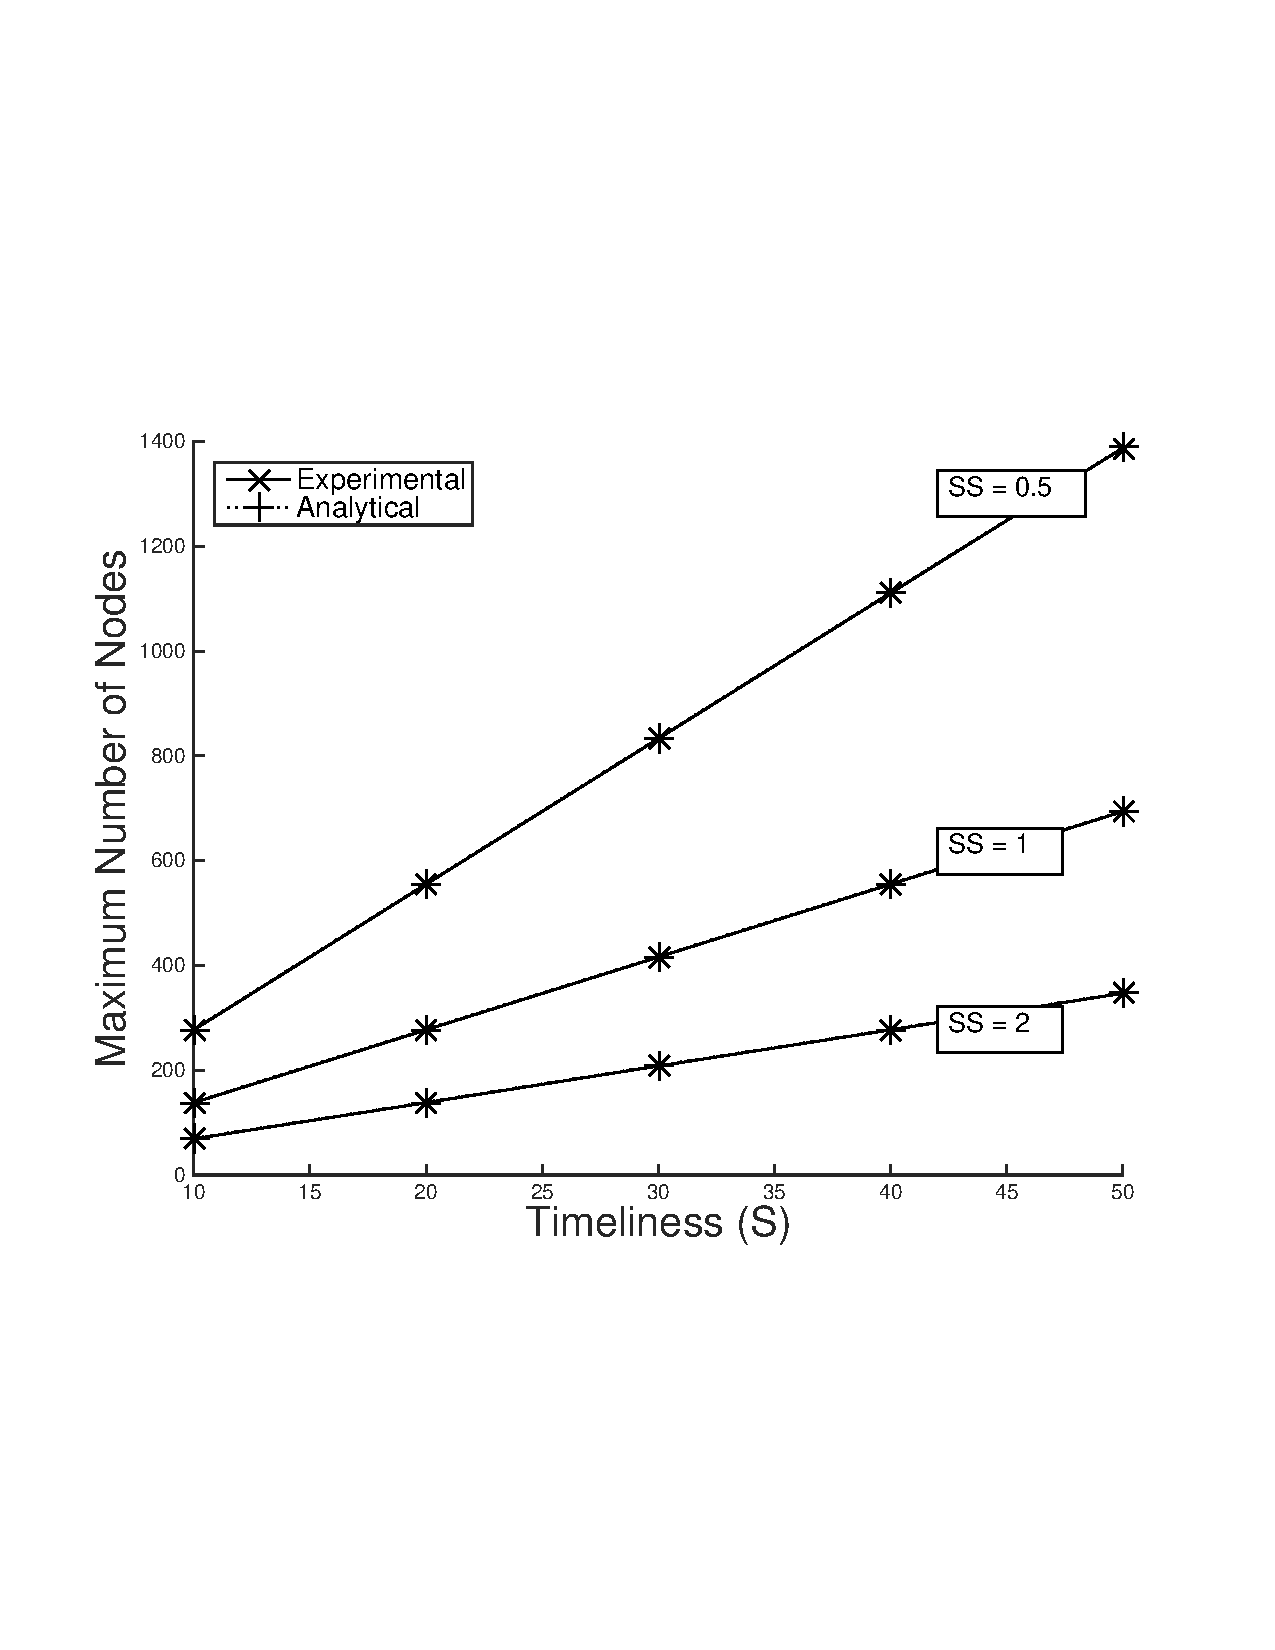
\includegraphics[scale=0.4, clip=true, trim=15mm 65mm 20mm 65mm]{figures/scal_sim_results/clique_uni_2d.pdf}
        \label{fig:scal_vs_qoi_clique}
        }
    \subfigure[Line Network, $I_S = 12 MB$]{
        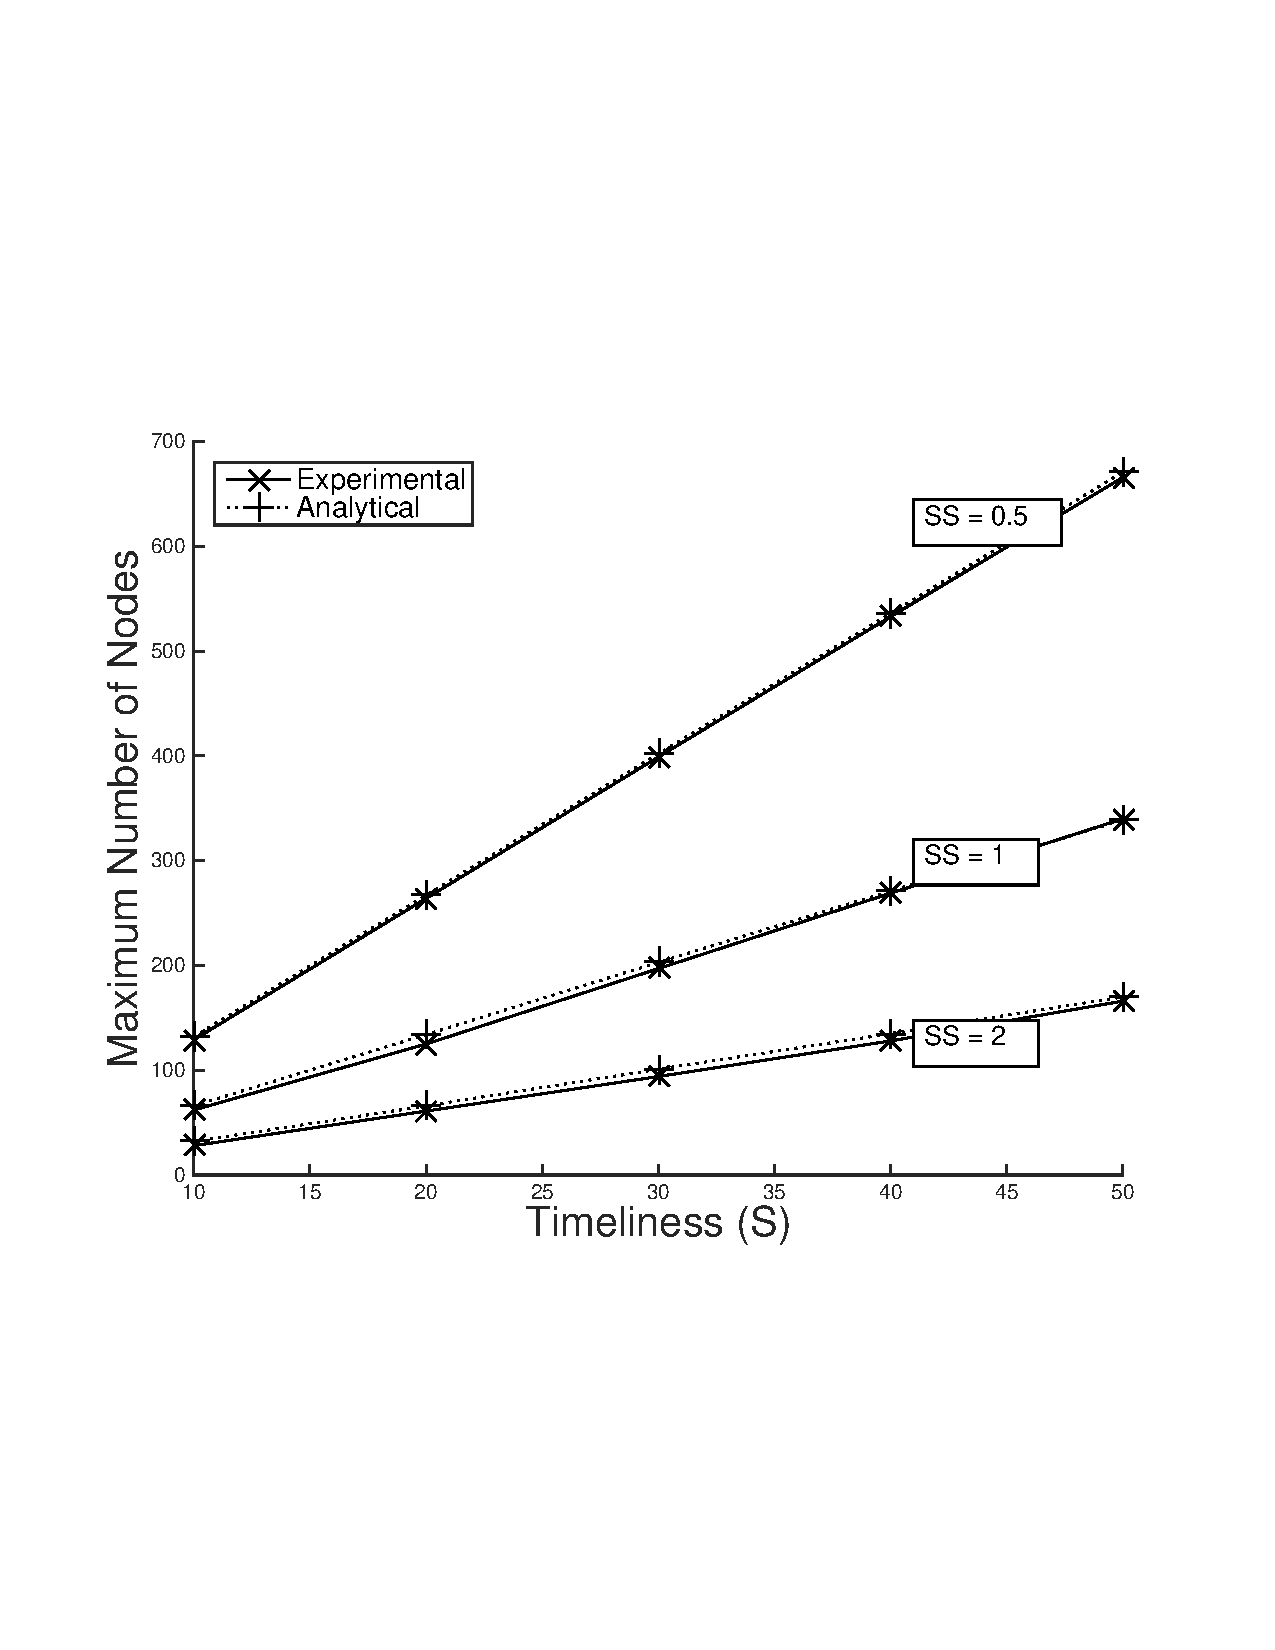
\includegraphics[scale=0.4, clip=true, trim=15mm 65mm 20mm 65mm]{figures/scal_sim_results/line_uni_2d_mhop_2.pdf}
        \label{fig:scal_vs_qoi_line}
        }
    \subfigure[Grid Network, $I_S = 48 MB$]{
        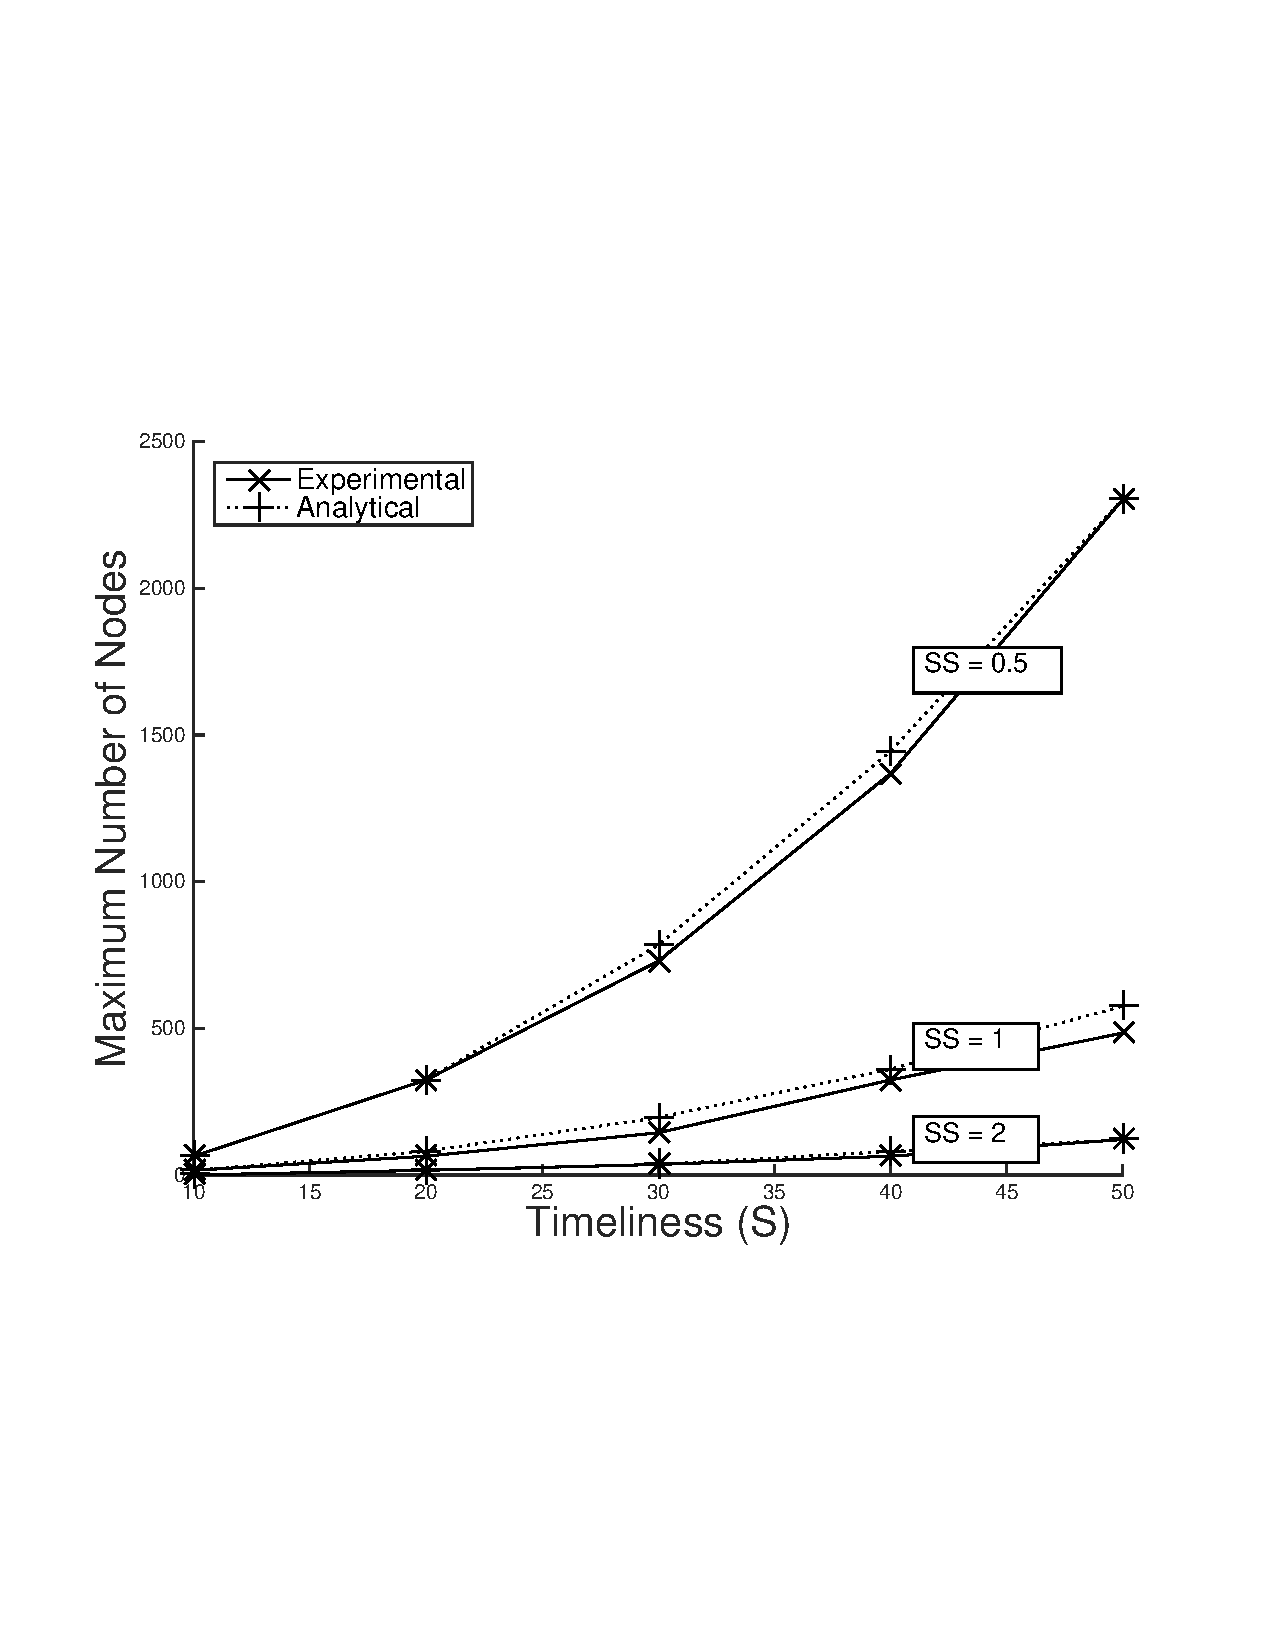
\includegraphics[scale=0.4, clip=true, trim=15mm 65mm 20mm 65mm]{figures/scal_sim_results/grid_uni_2d_mhop_2.pdf}
        \label{fig:scal_vs_qoi_grid}
        }
   \caption{Scalability vs. QoI Requirements}
   \label{fig:scal_vs_qoi}
\end{figure}

To show how effective estimates using this framework can be, we simulated the network topologies and traffic described above in Section \ref{sec:example_apply_fw} in the ns3 network simulator, comparing empirical results to those generated analytically.  We present a subset of these comparisons to provide evidence of the effectiveness of the methodology.  All results generated, however, exhibit very similar trends of proximity between empirical and the analytical values.

We use a channel rate of $W= 2 Mbps$, packet sizes of $P_s = 1500$ bytes, and image sizes of 9, 12, and 48 Mbytes.  As above, the correlation between Sum Similarity and $k_{req}$ is taken from the actual observed relation in Figure \ref{fig:topkSumSim}.  All values of parameters ($SS$, $T$, $I_S$, etc.) were chosen to test a variety of network sizes and QoI requirements while remaining within realistic network sizes, both with respect to real-world deployments and simulations with feasible run-times.%, e.g., network sizes over 2,500 nodes are outside of the scope of this paper's applications.  

Figure \ref{fig:scal_vs_qoi} shows the maximum scalability projected by solving inequalities \ref{eq:clique_gen}-\ref{eq:grid_gen} and the maximum scalability observed in our experiments.  In our simulations, we defined \emph{scalable} as a network in which all of the requested queries were entirely fulfilled within the specified timeliness requirement.  Small differences arise due to average values being used for $CF$, $TF$, $DF$, and $PL$, but, as the graphs show, in all of these scenarios, our network size estimates are very close to those realized in practical simulations.



%Figure \ref{fig:qoi_vs_num_nodes_grid} shows the same comparison, except displaying the maximum sum similarity values achievable for a fixed network size and several different timeliness constraints.  Many of the experimental results align exactly with the analysis.  Of those that differ from the projected achievable values, the gap between the points represents the smallest possible error, since the sum similarity is given as a set of discrete points based on the value of $k_{req}$.  In other words, the estimated sum similarity values are virtually all exactly on or exhibit the smallest possible error value.
%
%\begin{figure}
%\centering
%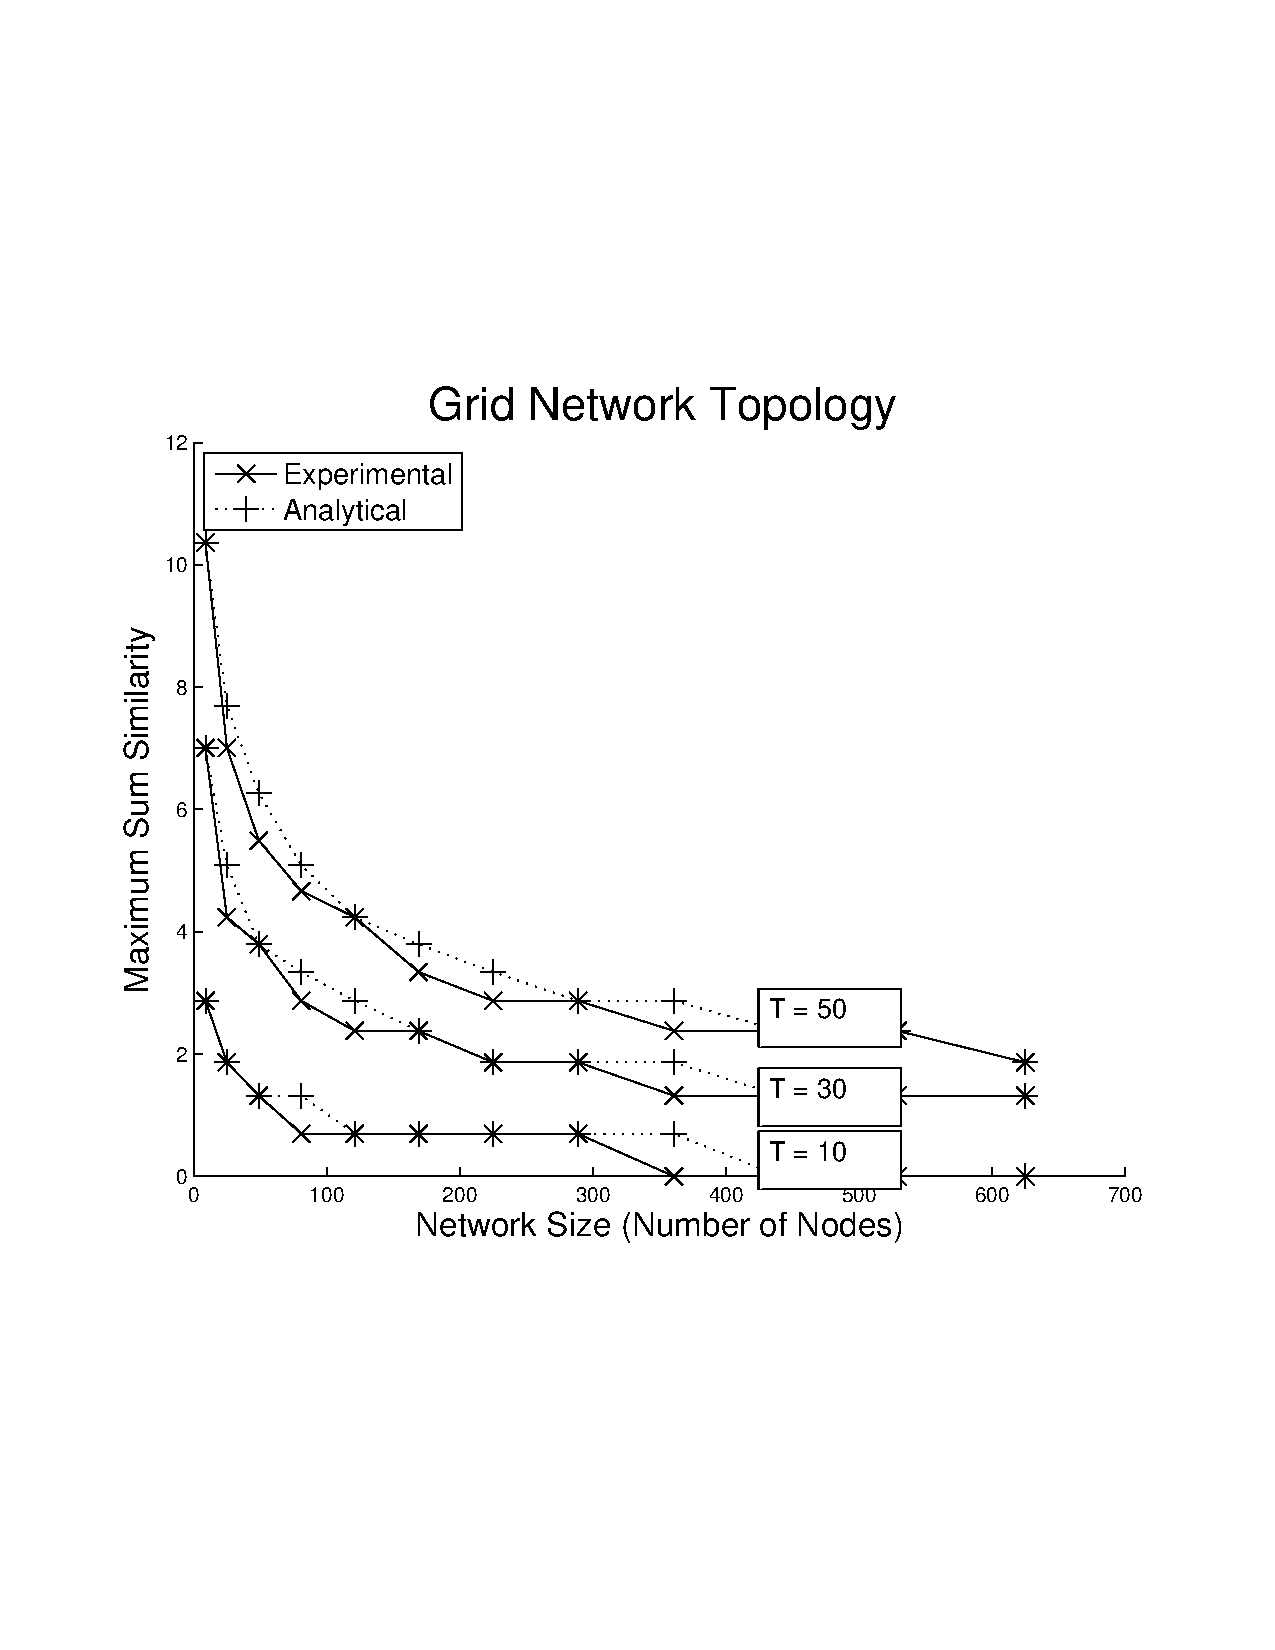
\includegraphics[scale=0.45, clip=true, trim=15mm 65mm 20mm 65mm]{figures/scal_sim_results/grid_max_ss_24_IS.pdf}
%    \label{fig:qoi_vs_num_nodes_grid}
%   \caption{Grid Network: Maximum Achievable QoI for Given Network Size}
%\end{figure}










